\documentclass[a4paper,12pt]{article}
\usepackage[a4paper, margin=1in]{geometry} % Sets the paper size to A4 and margins to 1 inch
\usepackage{graphicx}
\usepackage{subcaption} % for subfigures
\usepackage{setspace}		
\usepackage{xcolor,listings} % for typesetting code
\usepackage{enumitem}
\usepackage{tabularx}

% Define SQL listing style
% \lstset{
%     language=SQL,
%     basicstyle=\ttfamily,
%     keywordstyle=\bfseries,
%     commentstyle=\itshape,
%     showstringspaces=false,
%     numbers=left,
%     numberstyle=\tiny,
%     numbersep=5pt,
%     breaklines=true,
%     frame=single,
%     backgroundcolor=\color{gray!10},
%     captionpos=b
% }
\lstset{
    upquote=true,
    language=SQL,
    showspaces=false,
    basicstyle=\ttfamily,
    keywordstyle=\bfseries\color{blue!60},
    numbers=left,
    numberstyle=\tiny,
    commentstyle=\color{gray},
    backgroundcolor=\color{gray!10}
}

\begin{document}


%% Adding logo
\begin{figure}[h]
		\vspace*{-1em}
		\centering
		
\includegraphics[width=0.2\linewidth]{university_logo.png}
		\par
		\vspace*{2em}
		{\Large UNIVERSITY OF CHITTAGONG}
\end{figure}
%% Document information
\begin{center}
		\vspace*{3em}
		\textbf{Department of Computer Science and Engineering} \\
		\bigskip
		Session: 2021-2022 \\
		4th semester \\
		\bigskip
		\begin{tabular}{l l}
		  Assignment No. &: 1\\
		  Course Title &: Database Systems \\
		  Course Code No. &: CSE-413 \\
		\end{tabular}
\end{center}

%% Teacher information
\begin{center}
		\vspace*{3em}
		Submitted to: \\
		\textbf{Dr. Rudra Pratap Deb Nath} \\
		Associate Professor \\
		Department of Computer Science and Engineering \\
		University of Chittagong
\end{center}

%% Student information
\begin{center}
		\vspace*{3em}
		Submitted by: \\
		\textbf{Sanzid Islam Mahi} \\
		ID: 22701065 \\
		Department of Computer Science and Engineering \\
		University of Chittagong
\end{center}




\begin{center}
	\vspace*{3em}
	Date: Jul 02, 2024
\end{center}

\newpage
\section*{Chapter 6}
\subsection*{Practice 6}
\begin{enumerate}
    \item Write a query for the HR department to produce the addresses of all the departments. Use the
LOCATIONS and COUNTRIES tables. Show the location ID, street address, city, state or
province, and country in the output. Use a NATURAL JOIN to produce the results.

    \begin{figure}[h]
        \centering
            \centering
            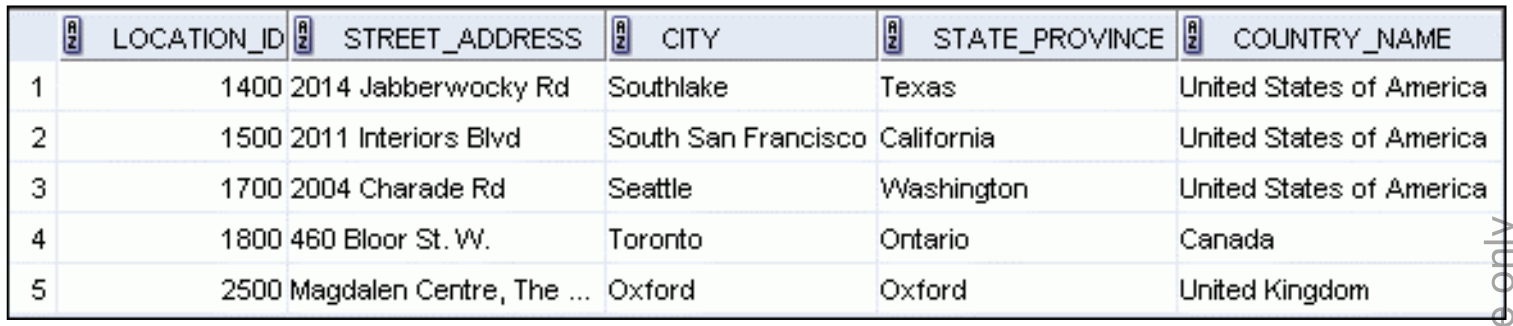
\includegraphics[width=.6\linewidth]{graphics/61.png}
    \end{figure}
    
    \textbf{Solution: }
    \begin{lstlisting}[language=SQL]

    \end{lstlisting}
        \item The HR department needs a report of all employees. Write a query to display the last name,
department number, and department name for all the employees.
    \begin{figure}[h]
        \centering
            \centering
            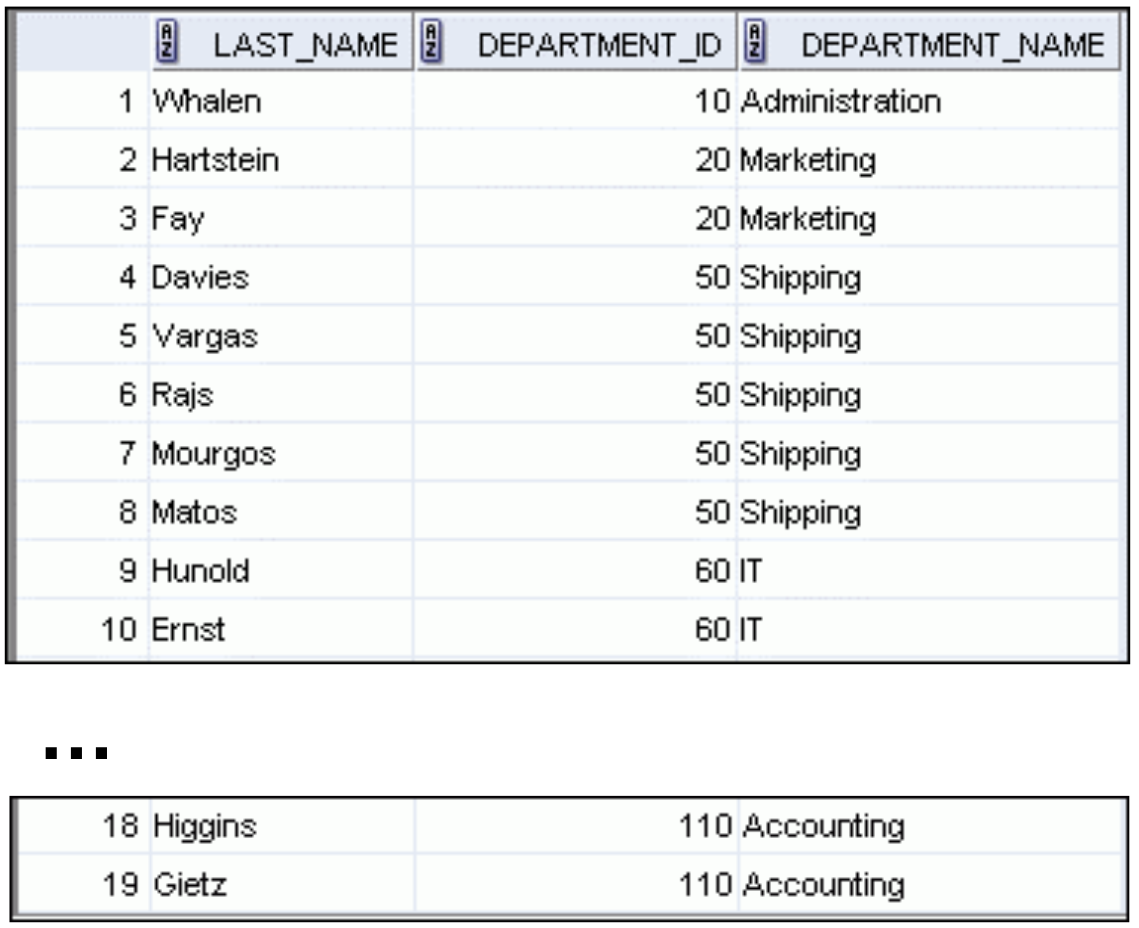
\includegraphics[width=.6\linewidth]{graphics/62.png}
    \end{figure}
    
    \textbf{Solution: }
    \begin{lstlisting}[language=SQL]

    \end{lstlisting}
    \newpage
    \item The HR department needs a report of employees in Toronto. Display the last name, job,
department number, and the department name for all employees who work in Toronto.
    \begin{figure}[h]
        \centering
            \centering
            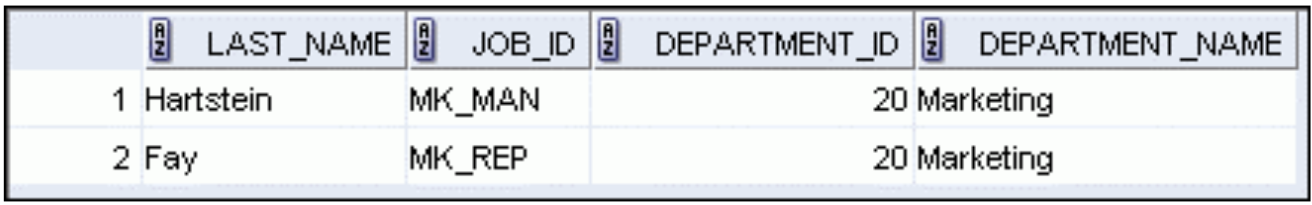
\includegraphics[width=.4\linewidth]{graphics/63.png}
    \end{figure}
    
    \textbf{Solution: }
    \begin{lstlisting}[language=SQL]

    \end{lstlisting}
        \item Create a report to display employees' last name and employee number along with their
manager's last name and manager number. Label the columns Employee, Emp\#, Manager,
and Mgr\#, respectively. Save your SQL statement as \texttt{lab\_06\_04.sql}. Run the query.
    \begin{figure}[h]
        \centering
            \centering
            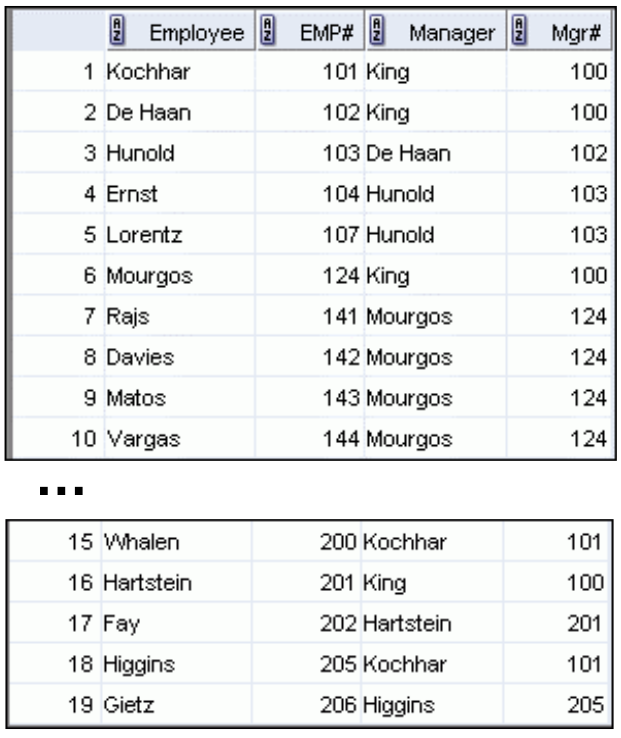
\includegraphics[width=.35\linewidth]{graphics/64.png}
    \end{figure}
    \newpage
    \textbf{Solution: }
    \begin{lstlisting}[language=SQL]

    \end{lstlisting}
    % \newpage
        \item \texttt{Modify\ lab\_06\_04.sql} to display all employees including King, who has no manager.
Order the results by the employee number. Save your SQL statement as \texttt{lab\_06\_05.sql}.
Run the query in \texttt{lab\_06\_05.sql}.
    
    \begin{figure}[h]
        \centering
            \centering
            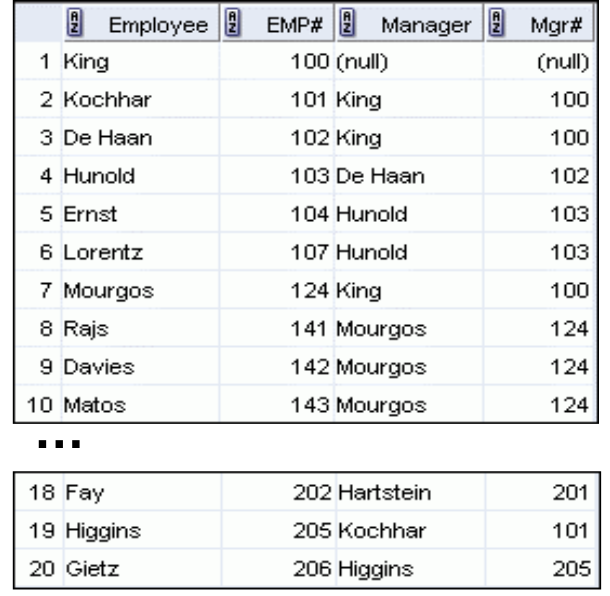
\includegraphics[width=.3\linewidth]{graphics/65.png}
    \end{figure}

    \textbf{Solution: }
    \begin{lstlisting}[language=SQL]

    \end{lstlisting}
    \newpage
    \item Create a report for the HR department that displays employee last names, department numbers,
and all the employees who work in the same department as a given employee. Give each
column an appropriate label. Save the script to a file named \texttt{lab\_06\_06.sql}.
    \begin{figure}[h]
        \centering
            \centering
            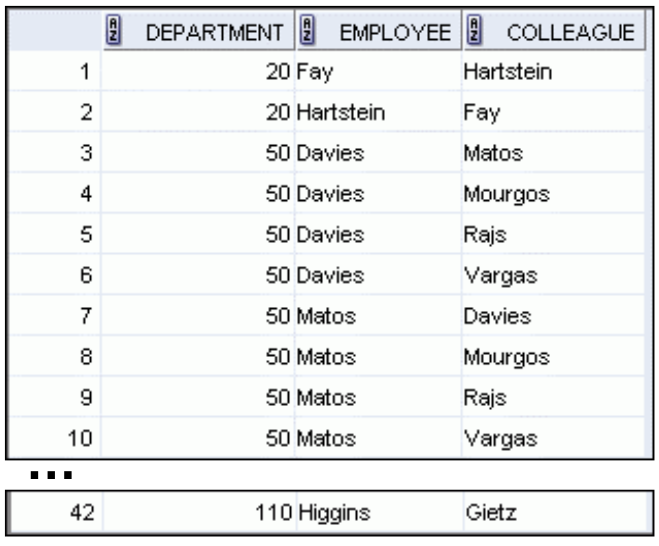
\includegraphics[width=.3\linewidth]{graphics/66.png}
    \end{figure}
    
    \textbf{Solution: }
    \begin{lstlisting}[language=SQL]

    \end{lstlisting}

        \item The HR department needs a report on job grades and salaries. To familiarize yourself with the
\texttt{JOB\_GRADES} table, first show the structure of the \texttt{JOB\_GRADES} table. Then create a query
that displays the name, job, department name, salary, and grade for all employees.
    
    \begin{figure}[h]
        \centering
            \centering
            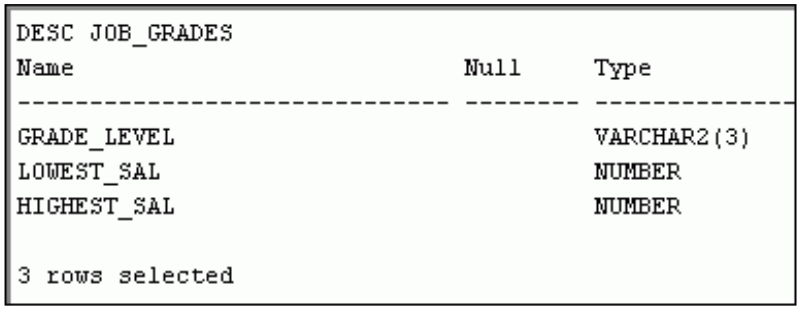
\includegraphics[width=.3\linewidth]{graphics/67.1.png}
    \end{figure}

    \textbf{Solution: }
    \begin{lstlisting}[language=SQL]

    \end{lstlisting}
    \newpage
    \item The HR department wants to determine the names of all the employees who were hired after
Davies. Create a query to display the name and hire date of any employee hired after employee
Davies.
    \begin{figure}[h]
        \centering
            \centering
            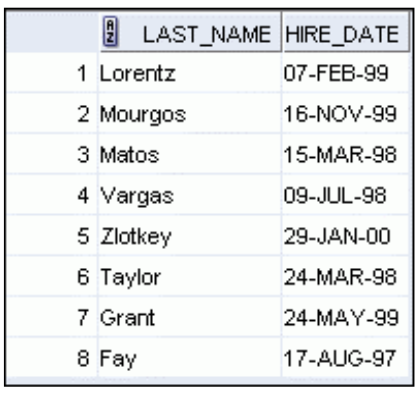
\includegraphics[width=.3\linewidth]{graphics/68.png}
    \end{figure}
    
    \textbf{Solution: }
    \begin{lstlisting}[language=SQL]


    \end{lstlisting}
    \item The HR department needs to find the names and hire dates of all the employees who were hired
before their managers, along with their managers' names and hire dates. Save the script to a file
named \texttt{lab\_06\_09.sql}.
    \begin{figure}[h]
        \centering
            \centering
            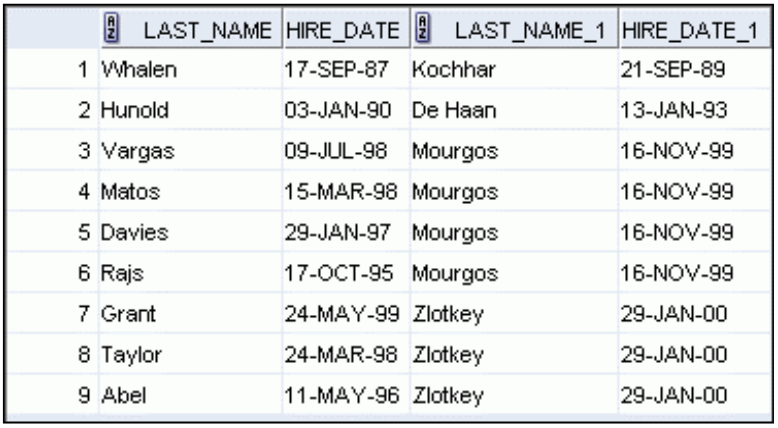
\includegraphics[width=.3\linewidth]{graphics/69.png}
    \end{figure}
    
    \textbf{Solution: }
    \begin{lstlisting}[language=SQL]


    \end{lstlisting}
\end{enumerate}










%%%%%%%% CHAPTER 7 %%%%%%%%


\section*{Chapter 7}
\subsection*{Practice 7}
\begin{enumerate}
    \item The HR department needs a query that prompts the user for an employee last name. The query
then displays the last name and hire date of any employee in the same department as the
employee whose name they supply (excluding that employee). For example, if the user enters
Zlotkey, find all employees who work with Zlotkey (excluding Zlotkey).

    \begin{figure}[h]
        \centering
            \centering
            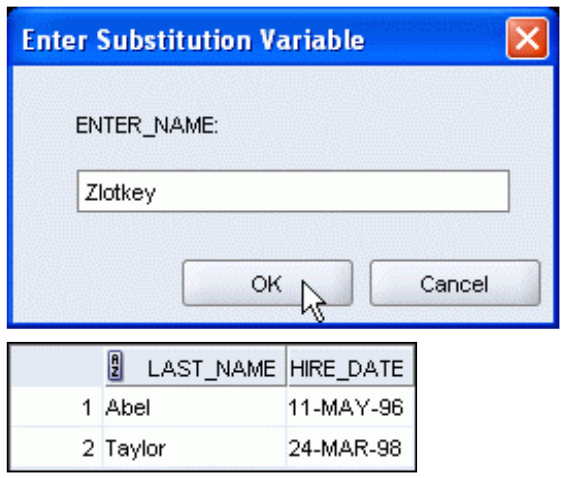
\includegraphics[width=.6\linewidth]{graphics/71.png}
    \end{figure}
    
    \textbf{Solution: }
    \begin{lstlisting}[language=SQL]

    \end{lstlisting}
        \item Create a report that displays the employee number, last name, and salary of all employees who
earn more than the average salary. Sort the results in order of ascending salary.
    \begin{figure}[h]
        \centering
            \centering
            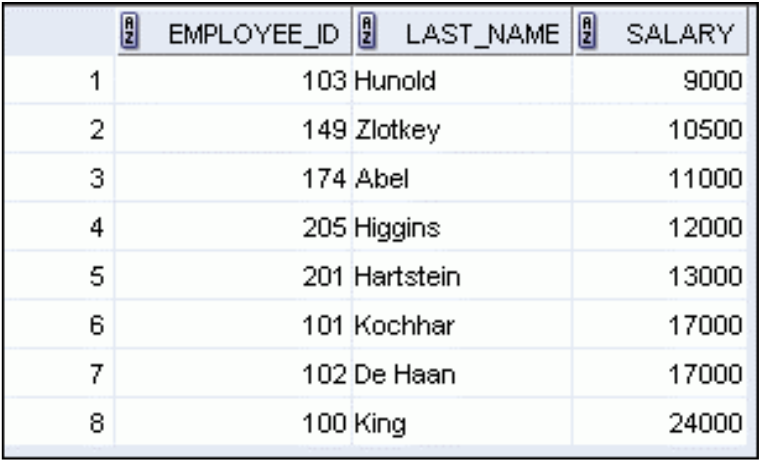
\includegraphics[width=.6\linewidth]{graphics/72.png}
    \end{figure}
    
    \textbf{Solution: }
    \begin{lstlisting}[language=SQL]

    \end{lstlisting}
    \newpage
    \item Write a query that displays the employee number and last name of all employees who work in a
department with any employee whose last name contains the letter “u.” Save your SQL
statement as \texttt{lab\_07\_03.sql}. Run your query.
    \begin{figure}[h]
        \centering
            \centering
            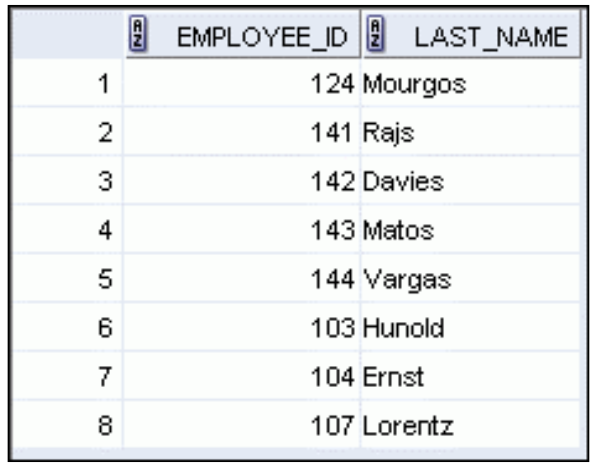
\includegraphics[width=.4\linewidth]{graphics/73.png}
    \end{figure}
    
    \textbf{Solution: }
    \begin{lstlisting}[language=SQL]

    \end{lstlisting}
        \item The HR department needs a report that displays the last name, department number, and job ID
of all employees whose department location ID is 1700.
    \begin{figure}[h]
        \centering
            \centering
            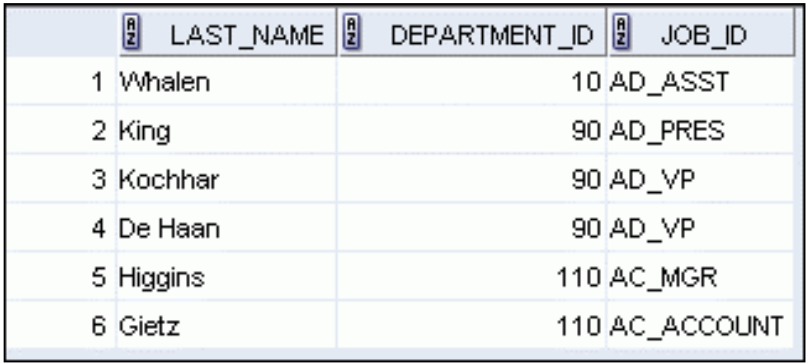
\includegraphics[width=.35\linewidth]{graphics/74.png}
    \end{figure}
    Modify the query so that the user is prompted for a location ID. Save this to a file named
\texttt{lab\_07\_04.sql}.
    \newpage
    \textbf{Solution: }
    \begin{lstlisting}[language=SQL]

    \end{lstlisting}
    % \newpage
        \item Create a report for HR that displays the last name and salary of every employee who reports to
King.
    
    \begin{figure}[h]
        \centering
            \centering
            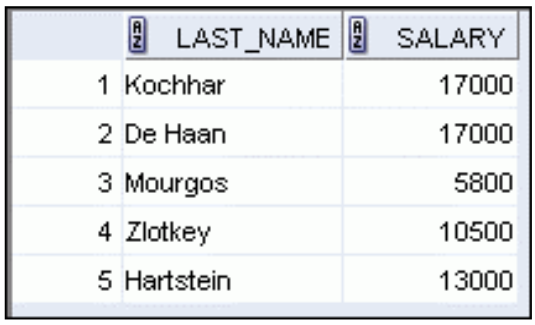
\includegraphics[width=.3\linewidth]{graphics/75.png}
    \end{figure}

    \textbf{Solution: }
    \begin{lstlisting}[language=SQL]

    \end{lstlisting}
        \item Create a report for HR that displays the department number, last name, and job ID for every
employee in the Executive department.

    
    \begin{figure}[h]
        \centering
            \centering
            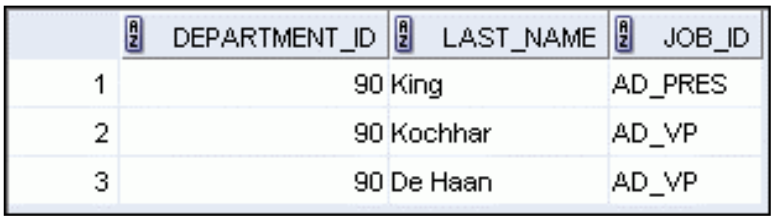
\includegraphics[width=.3\linewidth]{graphics/76.png}
    \end{figure}

    \textbf{Solution: }
    \begin{lstlisting}[language=SQL]

    \end{lstlisting}
        \item Modify the query in \texttt{lab\_07\_03.sql} to display the employee number, last name, and salary
of all employees who earn more than the average salary, and who work in a department with
any employee whose last name contains a ``u." Resave \texttt{lab\_07\_03.sql} as
\texttt{lab\_07\_07.sql}. Run the statement in \texttt{lab\_07\_07.sql}.

    
    \begin{figure}[h]
        \centering
            \centering
            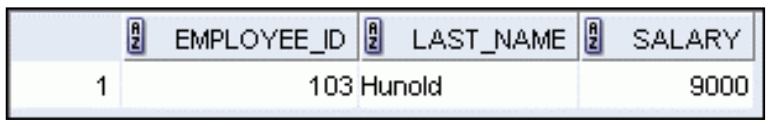
\includegraphics[width=.3\linewidth]{graphics/77.png}
    \end{figure}

    \textbf{Solution: }
    \begin{lstlisting}[language=SQL]

    \end{lstlisting}
\end{enumerate}

\end{document}
